% -*- root: ../main.tex -*-

% In questa sezione devono essere chiariti i compiti svolti da ciascun candidato nel caso in cui il gruppo abbia più di un componente. Deve essere inoltre esposto il piano di lavoro adottato. A tal fine, per ogni attività svolta durante la preparazione dell'elaborato (ad esempio: studio di una tecnologia, progettazione di un componente, implementazione di un algoritmo ecc. . . ) deve essere chiarita la collocazione temporale e devono essere indicate le risorse impiegate per svolgerla (giorni/uomo). I candidati possono ricorrere a opportuni diagrammi come quello di Gantt.
% 2000 - 4000 battute

\chapter{Piano di Lavoro}
Il piano di lavoro scelto ...
Diagramma di Gantt del lavoro svolto:
\begin{figure}[H]
    \caption{Gantt Chart del progetto}
    \label{fig:Gantt}] 
    \centering
   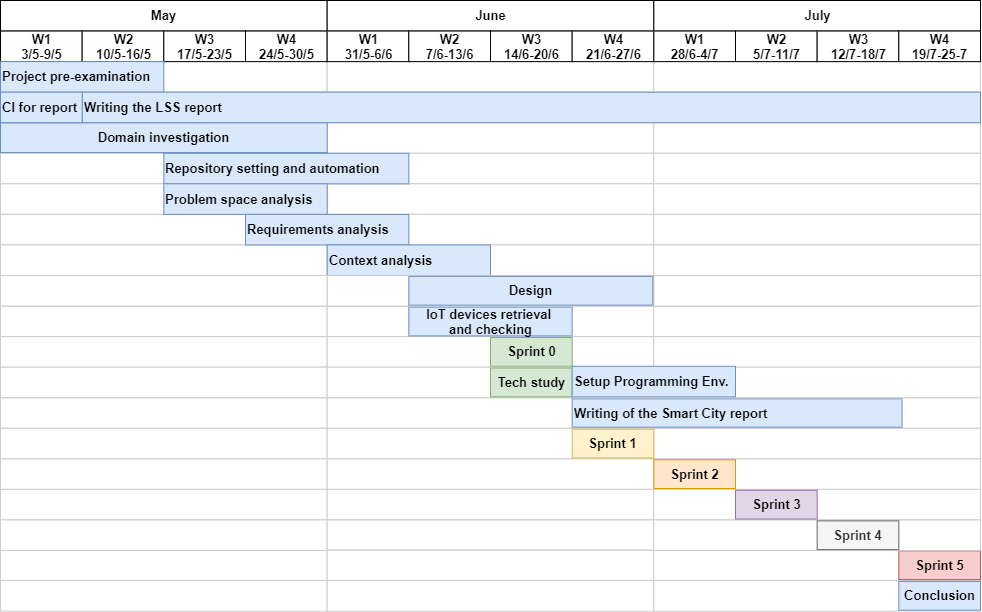
\includegraphics[width=1\textwidth]{DrawIo/GanttChart.png}
\end{figure}
